\documentclass[11pt]{report}  
\usepackage[T1]{fontenc}
\usepackage[utf8]{inputenc}
\usepackage{helvet}
\usepackage{titlesec} 
\usepackage[frenchb]{babel}
\usepackage{amsmath,amssymb}
\usepackage{tabu}
\usepackage[svgnames]{xcolor}
\usepackage{graphicx}
\usepackage{geometry}
\usepackage{layout}
\usepackage{listings}
\usepackage{textcomp}
\usepackage{minted}
\usepackage{pdfpages}

\newenvironment{strechpage}[1][0cm]{%
	\newpage\vspace*{#1}\leavevmode\noindent\centering
	\def\tempdimen{#1}%
	\begin{minipage}{\dimexpr\linewidth-#1-#1\relax}}%
	{\end{minipage}\vspace*\tempdimen\newpage}

\titleformat{\chapter}[display]
  {\centering\normalfont\huge\bfseries}
  {\chaptertitlename\ \thechapter}
  {20pt}
  {\Huge}
  
\newcommand\T{\rule{0pt}{2.6ex}}       % Top strut
\newcommand\B{\rule[-1.2ex]{0pt}{0pt}} % Bottom strut

\begin{document}
 \makeatletter
\def\maketitle{%
  \null
  \thispagestyle{empty}%
  \vfill
  \begin{center}\leavevmode
    \normalfont
    {\Huge \@title\par}%
    \vskip 3cm
    {\Large \@author\par}%
    \vskip 1cm
    {\Large \@date\par}%
  \end{center}%
  \vfill
  \null
  \cleardoublepage
  }
\makeatother
\title{Solution générique de calcul GRID exploitant des messageries instantanées
(Java / Python, XML, XMPP / IRC)}
\author{ Réalise par Joffrey Hérard \begin{center}Responsable : Olivier Flauzac\end{center}}
\date{2016-2017}
\maketitle
 
\tableofcontents 

\newpage
\chapter{Introduction} 
Sujet : Solution générique de calcul GRID exploitant des messageries instantanées
(Java / Python, XML, XMPP / IRC)
Durant ce TER, la mise en place d'un système de calcul repartie entre plusieurs machine avec l'évaluation de possibilité d'exécutions ou non par la machine cible, il fallait aussi évaluer quels échanges allais être réalise par les acteurs durant une exécution type et ceci en avec le protocoles XMPP ou IRC . 
\newpage
\chapter{Les Acteurs} 
Nous avons donc deux genres d'acteur pour chaque travail différent disponibles 
\begin{itemize}
\item Fournisseur de travail/Provider, unique pour chaque travail.
\item Des travailleurs/Workers, de 1 a n, n définit par le problèmes.
Chaque Provider est possiblement exécuter sur n'importe quel système d'exploitation  tout comme chaque worker
\end{itemize}
\newpage
\chapter{Les Échanges} 
Voici la liste des différents message qui transitent a travers une exécution type.
\begin{enumerate} \item Nous avons en premier le message de type "ENVOI JOB" il contient :
\begin{itemize}
\item l'identifiant du problème,
\item Le code des contraintes,
\item Le code a exécuter,
\item La ligne de  commande pour l\textquoteright exécuter.
\item Le nom du fichier à exécuter.
\end{itemize}
\item Ensuite il y a le message ou le workers signale qu'il est prêt il contiens juste un message pour signale dans une chaîne de caractère " Je suis prêt".
\item Il y a enfin le message qui renvoi le résultat "REPONSE JOB" il contient : 
\begin{itemize}
\item L'identifiant pour savoir si le code a pu être exécute.
\item L'identifiant du problème.
\item La valeur du retour de l\textquoteright exécution.
\item Code de contraintes, si on a pas pu exécuter .
\item Code exécutable, si on a pas pu exécuter .
\item Ligne de commande associe,  si on a pas pu exécuter .
\item Le nom du fichier à exécuter.
\end{itemize}
\end{enumerate}
Voici la liste des fichiers schéma XML associe ainsi que leurs locations au sein du projet :
\begin{itemize}
\item "ENVOI\_JOB" = ../Schema\_XML/ENVOI\_RECEPTION.xsd.
\item "REPONSE\_JOB"= ../Schema\_XML/JOB\_REP.xsd.

Tout les codes du projet sont présenter en annexe.
\end{itemize}

\newpage
\chapter{Les Erreurs} 
\section{Les Problèmes d'exécution}
Les problèmes qui peuvent opérer a travers le système,sont : 
\begin{enumerate}
\item Mauvais nom de domaine 
\item Problème de Chatroom déjà existante
\item Problème d'exécution : aucun worker peut exécuter le code, comment le détecter?

\end{enumerate}  

\newpage
\section{Les Problèmes réseaux}
Nous avons plusieurs problèmes lie au réseaux quelque soit le protocole utilise :
\begin{enumerate}
\item Latence/Impossible a établir une  connexion a la Chatroom
\item Latence/Impossible a envoyer un  message d'un Provider vers un Worker
\item Latence/Impossible a envoyer un  message d'un Worker vers un Provider
\item Un Worker est déconnecte en plein milieu de sa tache
\item Un Provider est déconnecte durant l'attente d'une réponse sur un JOB
\end{enumerate}
\newpage
\section{Gestions des erreurs}

\subsection{Gestions des erreurs sur l\textquoteright exécution}
\begin{enumerate}
\item Mauvais nom de domaine $ \rightarrow $ Redemander le nom de domaine jusqu'à validation .
\item Problème de Chatroom déjà existante $\rightarrow$ Message d'erreur un problème exactement identique est en cours d'exécution .
\item Problème d'exécution : aucun worker peut exécuter le code, comment le détecter? $\rightarrow$ Mis en place d'un tableau de variable booléenne au départ initialise a faux, si un worker renvoi avec une impossibilité d\textquoteright exécution du code dicte par le code contrainte, alors on met a vrai et on redistribue. Si aucun est capable on arrête l\textquoteright exécution.
\end{enumerate}  
\subsection{Gestions des erreurs sur le réseaux}
\begin{enumerate}
\item Latence/Impossible a établir une  connexion a la Chatroom$ \rightarrow $ Message qui explicite le fait d'aller voir un Administrateur Reseaux
\item Latence/Impossible a envoyer un  message d'un Provider vers un Worker$ \rightarrow $ Message qui explicite le fait d'aller voir un Administrateur Réseaux
\item Latence/Impossible a envoyer un  message d'un Worker vers un Provider$ \rightarrow $ Message qui explicite le fait d'aller voir un Administrateur Réseaux 
\item Un Worker est déconnecte en plein milieu de sa tache$ \rightarrow $ Détecteur de présence permis par le protocole XMPP sur une ChatRoom MultiUser
\item Un Provider est déconnecte durant l'attente d'une réponse sur un JOB$ \rightarrow $ Évaluation de présence d'un Provider, si aucun alors arrêter le Job en cours, ou mis en place d'un Timeout.
\end{enumerate}

\newpage
\chapter{Modélisation}
\section{Schéma général} 
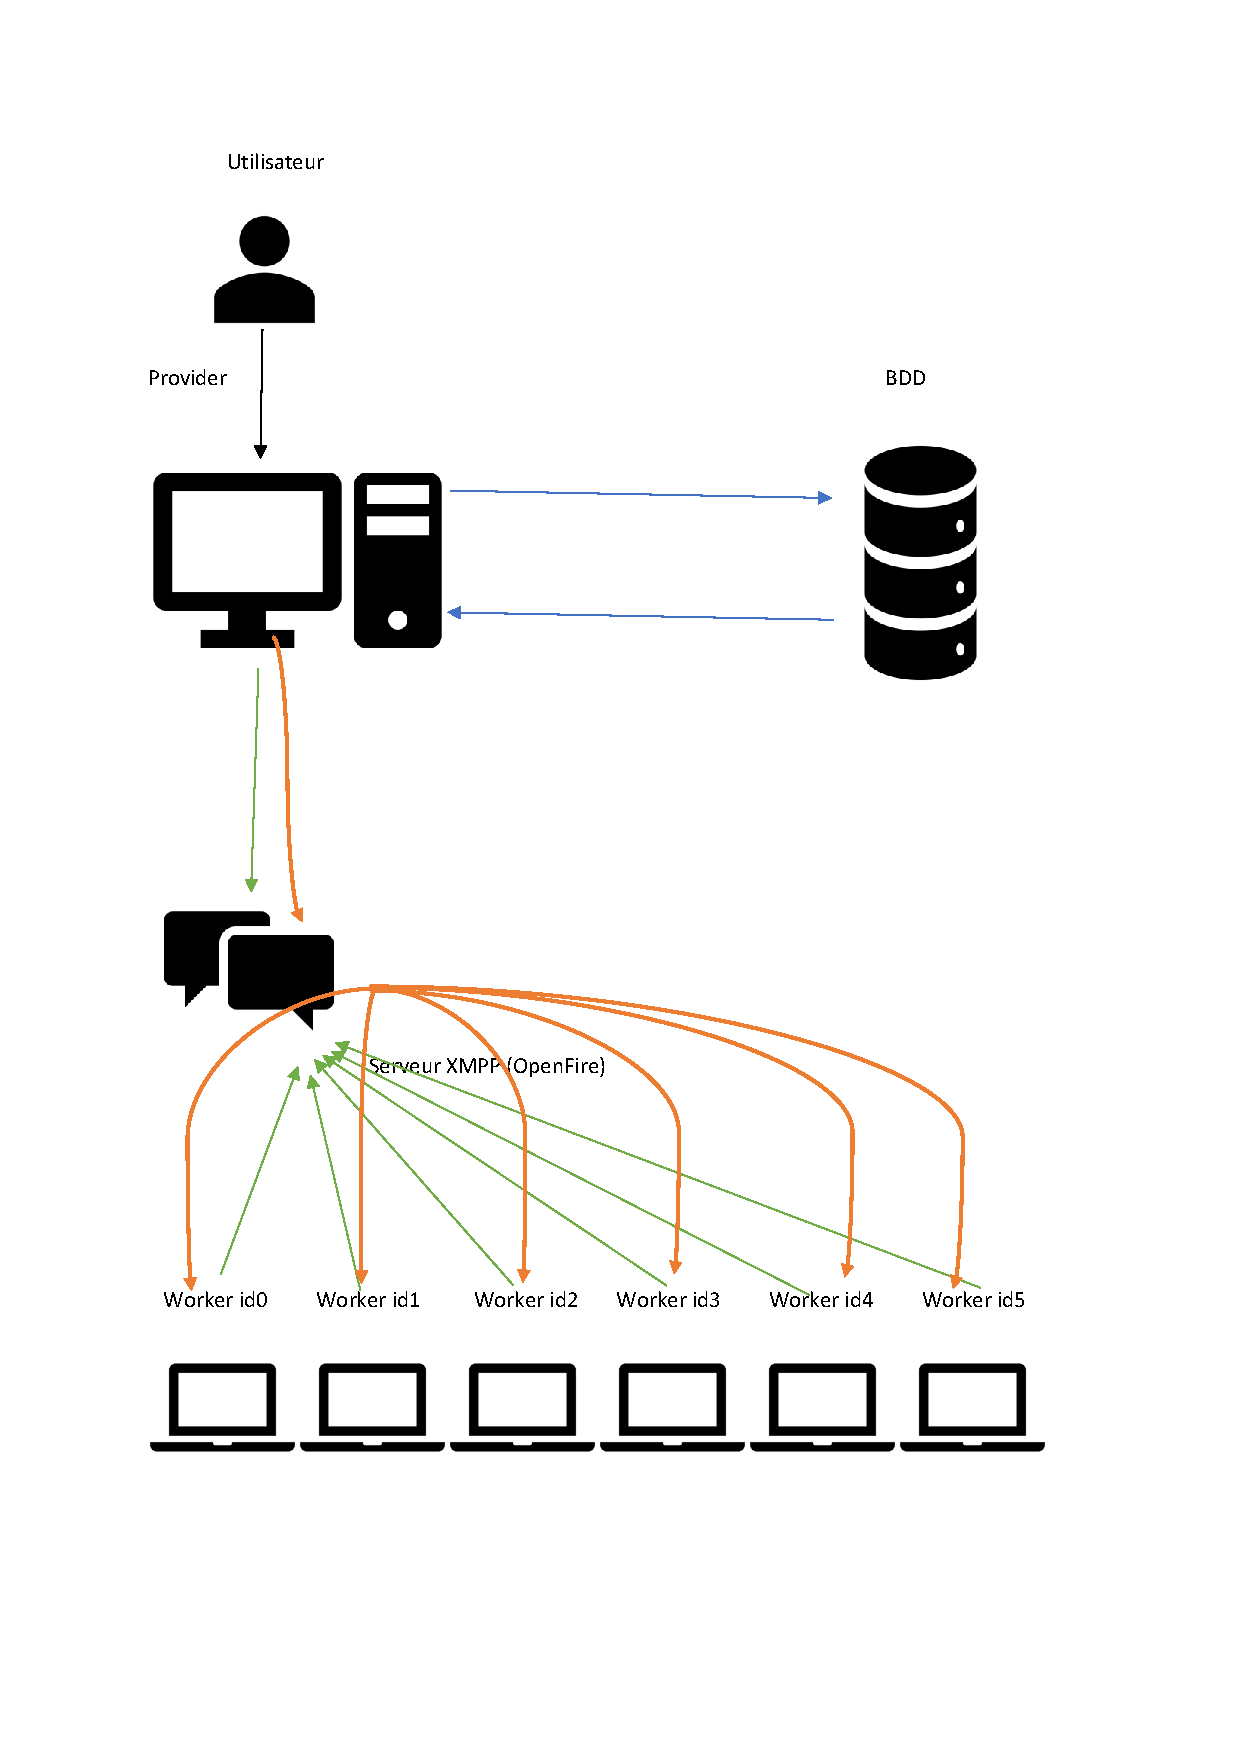
\includepdf[scale=0.7,pages=1,pagecommand=\subsection{Schéma global d'envoi d'un job}]{toto.pdf}
\includepdf[scale=1,pages=4]{toto.pdf}

\includepdf[scale=0.7,pages=2,pagecommand=\subsection{Schéma global d'envoi de réception d'un job}]{toto.pdf}
\includepdf[scale=1,pages=3]{toto.pdf}
\newpage
\section{Représentation des JOBS}
Nous allons dans cette partie du rapport montrer la représentation nécessaire et désirer pour représenter un travail.Donc un problèmes c'est quoi? 

\begin{itemize}
\item Identifiant d'un problème, un entier de 0 a n.
\item Code de contraintes, ce code est forcement un code Perl avec un code de retour bien particulier 0 pour non exécutable  et 3 pour exécutable et donc que l'on peut exécuter. 
\item Type du fichier par exemple ".c , .cpp, .cc, .java , .pl etc.."
\item Code d'exécution, peut importe son langage. on peut l'exécuter si le code contraintes l'a valider 
\item La ligne de commande pour exécuter le code par exemple "perl monfichier.pl"
\end{itemize}

\inputminted{XML}{../Schema_XML/BDD_JOB.xsd}
\newpage 

\section{Représentation des fichiers de lignes de commande} 
Chaque ligne de commande doit être représenter comme elle se doit c'est a dire la commande puis une ',' sinon, le parsing se faisant sur ce fichier par une expression régulière ne s\textquoteright appliquera pas correctement  
\inputminted{perl}{../Echantillon_Script_Cmd/Toto.dc}
Exemple de Langford\_mono12.dc :
\inputminted{perl}{../Echantillon_Script_Cmd/Langford_mono12.dc}
Exemple de nQueen14.dc :
\inputminted{perl}{../Echantillon_Script_Cmd/nQuenn14.dc}
\newpage
\section{Les différentes fonctions principales}

\subsection{Contraintes} 
L'execution d'un script de contrainte ce fait avec les objets Runtime et Process on obtient le résultat du script avec la fonctin waitFor() 
\inputminted{perl}{../Echantillon_Script_Perl/OSname.pl}
\newpage
\subsection{Split} 
La fonction split peut se résumer en plusieurs étapes, premièrement on récupère tout les nickname et JID de chaque utilisateur de la chatroom ,pour chacun d'entre eux on leur envoi un fichier xml personnalise avec chacun une tache bien distincte en respectant le schéma associe.Pour avoir une trace on sauvegarde chaque fichier xml envoyer dans le dossier JOB\_SEND
\inputminted[tabsize=2,frame=lines,linenos]{java}{Fichier_import/split.java}
\subsection{Exec} 
L\textquoteright exécution d'un script d'exécution ce fait avec les objets Runtime et Process on obtient le résultat du script avec la fonctin waitFor() bien entendu on parle de calcul chiffrer ,cela peut être aussi un résultat chiffre dans un fichier. 
\inputminted[tabsize=2,frame=lines,linenos]{Perl}{Fichier_import/calcul.pl}
\newpage
\subsection{Build} 
La fonction build est simplement une addition de chaque résultat reçu petit a petit 
\inputminted[tabsize=2,frame=lines,linenos]{java}{Fichier_import/build.java}
\newpage
\section{Description d'une exécution quelconque} 
\subsection{Exécution cote Provider}
Voici un déroulement classique cote Provider :
\begin{enumerate}
\item Un Provider choisi un problème a lancer.
\item Une fois le Problème lancer une Chatroom comportant le nom du problème+Providingroom est créer sur le domaine
\item Le Provider attend un nombre suffisant de Worker en fonction du probleme(champ rang du XML)
\item Une fois un nombre de Worker atteints, on récupère chaque identifiant et on leur envoi leur job respectif et ligne de commande respective
\item On attend d'avoir reçu un message de type "JOB\_Reponse" autant de fois et distinct que de Workers capable de l'exécuter 
\item On affiche le résultat
\end{enumerate}

\subsection{Exécution cote Worker}
Voici un déroulement classique cote Worker
\begin{enumerate}
\item On s'identifie
\item On choisi un salle de travail 
\item une fois connecter on applique la même routine 
\item A savoir, on exécute chaque script de contrainte si ils sont valide on exécute le fichier exécutable avec la ligne de commande associe.
\end{enumerate}
\subsection{Exécution d'un ajout}
\begin{enumerate}
\item On demande le nom du problème 
\item On demande en entrer le chemin absolu pour un fichier de contrainte
\item On demande en entrer le chemin absolu pour un fichier exécutable
\item On demande en entrer le chemin absolu pour un fichier correspondant aux ligne de commande
\item On demande en entrer un rang qui est égale aux nombre de workers nécessaire 
\item Tout ceci est ajouter a un fichier XML nomme nom\_du\_probleme.xml
\end{enumerate}

\newpage\subsection{Exécution d'une suppression}
\begin{enumerate}
\item On demande le nom du problème 
\item On supprime le fichier XMl associe 
\end{enumerate}

\chapter{Formatage des fichiers sources décrivant un JOB}
\section{Script de contraintes}
\subsection{Principe}
Tout script de contraintes doit répondre a ces propres contraintes :
\begin{enumerate}
\item Être écrit en Perl
\item Avoir un retour de commande avec "exit(3);" pour un retour validant la poursuite du processus 

\end{enumerate}
\subsection{Exemple}
\subsubsection{Exemple pour un programme interpréter}
Pour un langage interpréter comme le python en voici un exemple
\inputminted{perl}{../Echantillon_Script_Perl/nqueen.pl}
\subsubsection{Exemple pour un programme compilé }
Quand il s'avère que vous devez valide la compilation puis sa future exécution d'un code exécutable tel q'un code de langage compilé comme le C en voici un exemple sur comment faire 
\inputminted{perl}{../Echantillon_Script_Perl/langford.pl}
\section{Script de Commandes}
\subsection{Principe}
Tout script de commande doit répondre a ces propres contraintes :
\begin{enumerate}
\item Après la commande faisant appelle a un interpréteur mettre le caractère "@"
\item Dans le cas d'un split a plus de 1 Worker, utiliser les virguler pour séparer chaque commande approprie pour chaque worker
\item Les caractères évidemment interdit sont : @, ',', [, ] .en raison d'exploitation d'expression régulière.
\end{enumerate}
\subsection{Exemple}
Voici quelques exemples :
\inputminted{perl}{../Echantillon_Script_Cmd/nQuenn14.dc}
\inputminted{perl}{../Echantillon_Script_Cmd/Toto.dc}
\section{Script de build}
\subsection{Principe}
Tout script de contraintes doit répondre a ces propres contraintes :
\begin{enumerate}
\item Être écrit en Perl.
\item Avoir connaissance que toutes les données renvoyer par les Worker seront passée en argument.
\item Écrire le résultat dans un fichier "resultatF.txt".
\end{enumerate}
\subsection{Exemple}
\inputminted{perl}{../Echantillon_Script_build/build.pl}
\chapter{Conclusion}


\chapter{Annexes}
\section{Organisation du Projet}
\begin{itemize}
\item / \begin{itemize}
		\item /bin  \begin{itemize} \item Tout les fichiers .class \item Images \item Schema    \end{itemize}
		\item /DB\_JOBS \begin{itemize} \item Calculatoire.xml \item Calculatoire2.xml \item Langford.xml \item etc.. \end{itemize}
		\item /Echantillon\_Script\_Cmd \begin{itemize} \item Robin.dc \item Toto.dc \item etc..\end{itemize}
		\item /Echantillon\_Script\_Exec \begin{itemize}\item calcul.pl  \end{itemize}
		\item /Echantillon\_Script\_Perl \begin{itemize}\item  DitributionContraintes.pl \end{itemize}
		\item /JDOM  
		\item /JOB\_REC \begin{itemize} \item \item /DATA\_EXTRACT \begin{itemize} \item fichier\_extraits\end{itemize}\item xml\_receive.xml  \end{itemize}
		\item /JOB\_SEND \begin{itemize}\item XML\_send\_0.xml \end{itemize}
		\item /openfire
		\item /Rapport \begin{itemize}\item TER\_Joffrey\_Herard.pdf  \end{itemize} 
		\item /Schema\_XML \begin{itemize}\item BDD\_JOB.xsd \item ENVOI\_RECEPTION.xsd \item JOB\_REP.xsd \end{itemize}
		\item /smack\_3\_1\_0
		\item /src \begin{itemize}\item Tout les fichiers .java \end{itemize}
		\item README.md 
\end{itemize}

\end{itemize}
\subsection{Outils et langages} 
\begin{enumerate}
\item Le projet a été programme en Java version : "1.8.0\_111" sous Eclipse  .
\item L'API smack a été utilisé pour mettre ne place les échanges sous XMPP.
\item Openfire a été utilisé pour installer un serveur XMPP en local afin d'exécuter tout les test.
\end{enumerate}
\newpage

\newpage
\section{Code}
\subsection{XML} 

BDD\_JOB.xsd
\inputminted[tabsize=2,frame=lines,linenos]{XML}{../Schema_XML/BDD_JOB.xsd}

ENVOI\_RECEPTION.xsd
\inputminted[tabsize=2,frame=lines,linenos]{XML}{../Schema_XML/ENVOI_RECEPTION.xsd}
\newpage
JOB\_REP.xsd
\inputminted[tabsize=2,frame=lines,linenos]{XML}{../Schema_XML/JOB_REP.xsd}
\newpage
\subsection{Fichier de lignes de commande .dc}
Les exemple de fichier de commande écrit en texte clair 
Toto.dc
\inputminted[tabsize=2,frame=lines,linenos]{Perl}{../Echantillon_Script_Cmd/Toto.dc}
\subsection{Perl}
Les exemple de fichier de contrainte écrit en Perl 
langford.pl
\inputminted[tabsize=2,frame=lines,linenos]{Perl}{../Echantillon_Script_Perl/langford.pl}

nqueen.pl
\inputminted[tabsize=2,frame=lines,linenos]{Perl}{../Echantillon_Script_Perl/nqueen.pl}
OSname.pl
\inputminted[tabsize=2,frame=lines,linenos]{Perl}{../Echantillon_Script_Perl/OSname.pl}

\end{document}